\documentclass[a4j,12pt,onecolumn,oneside,final]{jreport}

\usepackage[dvipdfmx]{graphicx}	%figure
\usepackage{subfig}
\usepackage{latexsym}
\usepackage[pdftex]{epstopdf}
%\usepackage{gthesis}
\usepackage{gthesis_myown}

\usepackage{amsmath,amsthm,amssymb,ascmac}
\usepackage{fancybox}
\usepackage{slashbox}
%\usepackage[dviout]{color,graphics}
\usepackage{graphicx}
\usepackage{color}
\usepackage{psfrag}
%\usepackage{upgreek}
\usepackage{bm}
\usepackage{wrapfig}

%%%%%%%%%%%%%%%%%%%%%%%%%%%%%%%%%%%%%%%%%%%%%%%%%%%%%%%%%%%%%%%%
% put local tex-macros in this file %

%%%%%%%%%%%%%%%%%%%%%%%%%%%%%
%色設定
%%%%%%%%%%%%%%%%%%%%%%%%%%%%%
\definecolor{Black}{rgb}{0.0,0.0,0.0}
\definecolor{Red}{rgb}{0.9,0.0,0.1}
\definecolor{Blue}{rgb}{0.1,0.1,0.5}
\definecolor{Green}{rgb}{0.1,0.4,0.1}
\definecolor{Gray}{rgb}{0.75,0.85,0.9} % Fuji-iro
\definecolor{Shade}{rgb}{0.1,0.1,0.4}

%%%%%%%%%%%%%%%%%%%%%%%%%%%%%%%%%%%%%%%%%%%%%%%%%%%%%%%%%%%%%%%%
\年度{平成26年度}
%\提出年月{平成26年7月}
\提出年月{平成27年2月}

\題名{SIBM - RDF形式に記述した避難場所情報\\ベンチマークツール}
\梗概題名{SIBM - RDF形式に記述した避難場所情報\\ベンチマークツール}
%\題名{楽に卒業する方法に関する基礎的研究\\
%			--- そもそもそれは可能か? ---}
%\梗概題名{楽に卒業する方法に関する基礎的研究\\
%			--- そもそもそれは可能か? ---}

\指導教員名A{横田 治夫}
\職名A{教授}

\指導教員名B{荒堀 喜貴}
\職名B{准教授}

%\所属学科{電気電子工学科}{}
\所属学科{情報工学科}{}
\学籍番号{11\_27820}
\氏名{NGUYEN Hoai Nam}

\内容梗概{
世界中で毎年、災害による損失や市民生活への影響が問題となっている.災害発生時には、避難情報を元に避難することが必要であるが、
災害発生後に、避難に関する情報やデータの量は急速に増加する.このため、適切な災害・避難情報の管理が求められる.

一方、近年RDF形式で記述されたデータが幅広く使用され、災害情報などを含む様々なデータがRDF形式で保存されることが増えている.
RDF形式を利用すると、情報の細かな管理やアクセス制限を適切に行うことができるが、既存の災害情報のRDF表現では、被災者個人間の関係や
被災者と医者、ボランティアなどの支援者との関係や、どの支援者がどの被災者にどのような作業を行って良いかといった関係を表現できていない.

そこで、本研究では、これらの詳細な関係をRDF形式で記述した災害・避難情報のデータセットSIBMを提案する.
SIBMの目的は、被災地における被災者-支援者間のデータ共有方式の妥当性の評価を可能にすることである.
具体的には、被災者の怪我の程度などの個人情報は医療従事者にのみ開示し、他の被災者には個人情報へのアクセスを許可しないなどの
データ共有方式の性能や秘匿情報保護能力をSIBMによって計測できるようになることを目指す.}

\begin{document}
% ----------------------------------------------------------------------
% 表紙
\maketitle
% ----------------------------------------------------------------------
% 目次
\setcounter{page}{1}
\renewcommand{\thepage}{\roman{page}}
\setcounter{tocdepth}{1}
\tableofcontents
\clearpage
% ----------------------------------------------------------------------
% 内容
\setcounter{page}{1}
\renewcommand{\thepage}{\arabic{page}}
%\chapter{Introduction}
\chapter{序論}
全世界には 、毎年災害が沢山発生する.大規模災害の2011年の大震災の他 、台風による災害事故や土砂災害などによる破壊が多いとわかった.
災害が発生するとき、避難することは重要である.避難する際、避難場所情報の管理や、避難する作業に関係のある人々の情報が多量に増加することがある.
それらの情報を管理・アクセスすることが重要な作業である.現実では、避難することに関する情報の中に、避難場所情報、
避難する人の情報、避難場所で作業する人(アシスタント・ボランチアなど)の情報があり、それらの情報を管理・アクセスすることが考えられる.
災害が発生するとき、それらの情報に対してすぐに対応できることが重要である. そのため、災害対策作業に対して、
現実に近い情報を使用しながら実験することは実際の要求である.

	一方、近年には、様々な新たなデータ記述法が開発されている.その中に、RDF形式で記述されたデータが増えている.
RDF形式で記述された避難・災害情報を公開・管理することが考えられている\cite{cite:opendata}.
RDF形式で記述したデータが、情報へのアクセス範囲をさらに細かく設計できることがわかる.避難作業情報の中に、
そのようなアクセス制限モデルが必要であり、共有範囲を限定すべき情報を暗号化することが現実の問題である.
例えば、避難作業の関係者の中に、避難者にみせられない情報や個人情報の秘密性に応じるアクセス範囲の制限が必要と考えられる\cite{cite:kodama}.
また、災害が発生するとき、情報がだんだん増加することがわかる.多量データを暗号化することも考えられる.
そこで、効率的に暗号化する手順が必要である\cite{cite:dat}.

	上記の問題に対して、RDF形式で記述した避難する作業に関するデータセットを使用して様々な使用シナリオで実験する要求がある.
本稿では、RDF形式で記述された避難場所情報と避難作業情報を生成するベンチマークツール - SIBM - を実装する.
そして、実装したベンチマークツールの構成、実験環境と実用例について考察する.

%\chapter{Preliminaries}
\chapter{準備}

\section{RDFについて}
\label{knowlegde:rdf}

\textbf{RDF(Resource Description Framework)}は、WWW上で資源に関する情報を表わすための言語である.
タイトル、著者、ウェブ・ページの更新日、ウェブ・ドキュメントの著作権およびライセンス情報、
ある共有資源に対する利用可能スケジュールなどのような、ウェブ資源に関するメタデータの表現を特に目的としている.
\footnote{http://www.asahi-net.or.jp/~ax2s-kmtn/internet/rdf/rdf-primer}
RDF形式で記述された情報がトリプル(図\ref{fig:rdf_triple}のA)あるいはRDFグラフ(トリプルの集合)(図\ref{fig:rdf_triple}のB)で表現できる.

\begin{figure}[h!]
 	\begin{center}
 		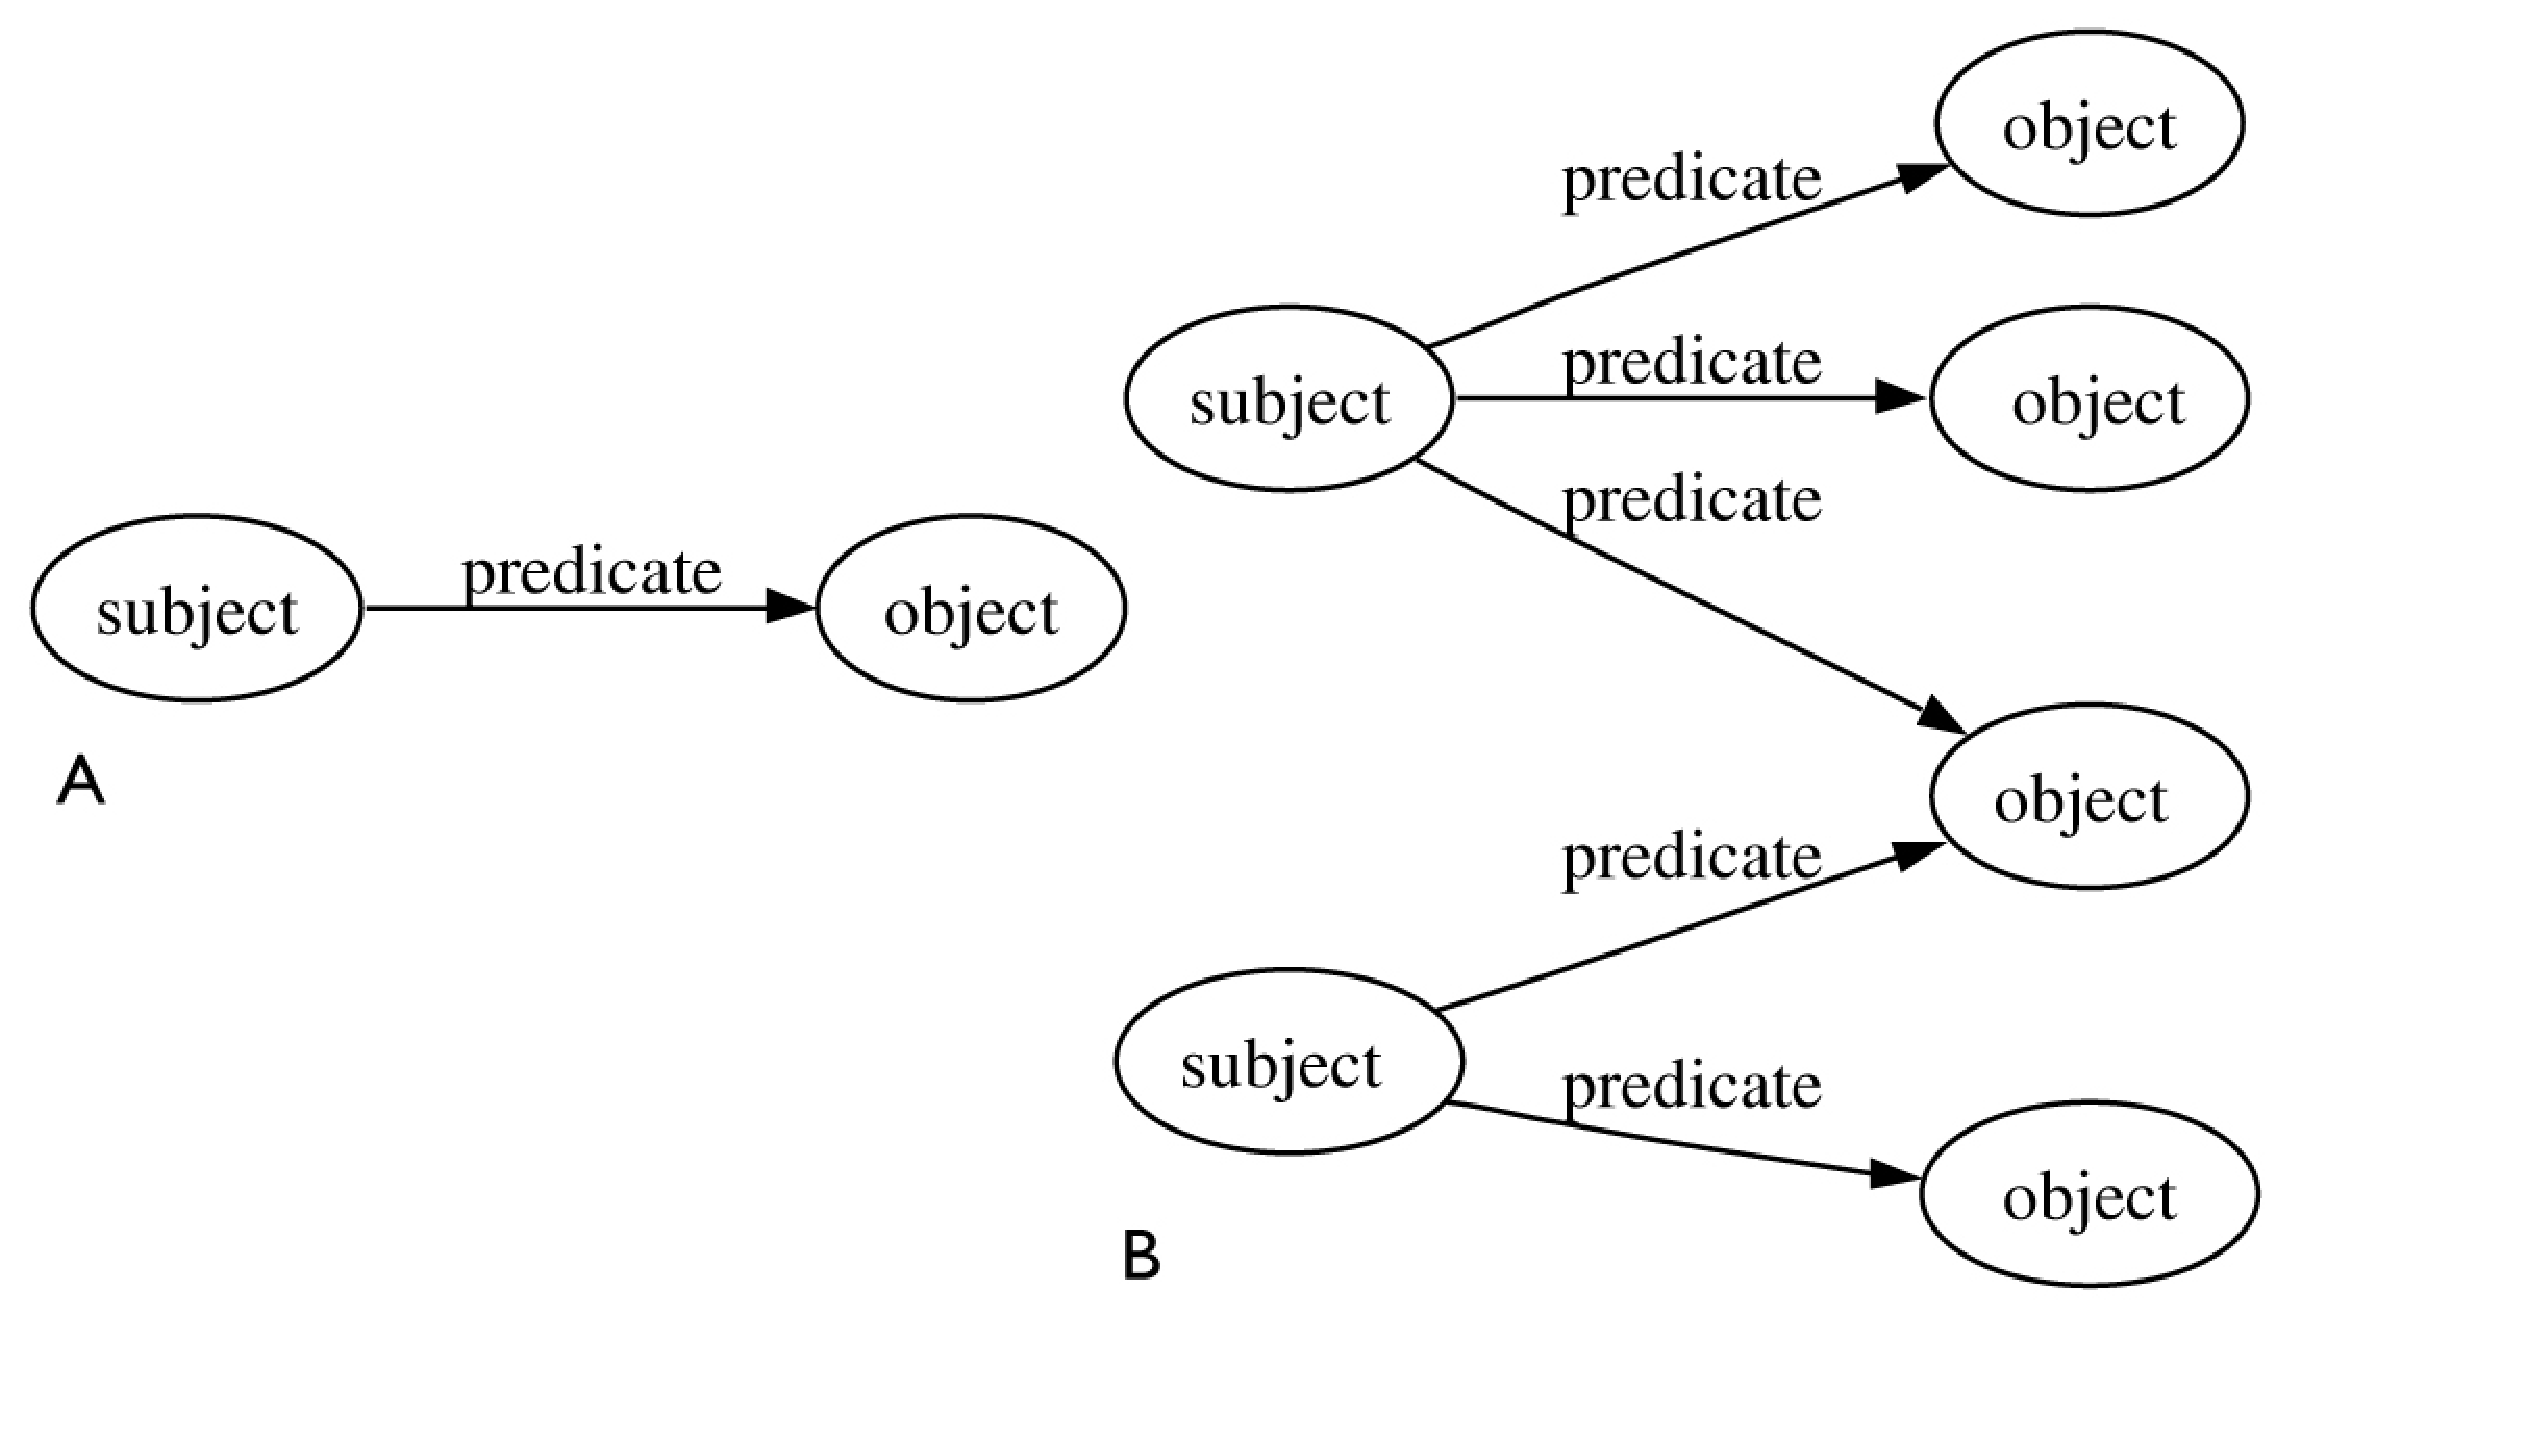
\includegraphics[width=160mm]{./images/rdf_sample.eps}
 		\caption{RDFの例}
 		\label{fig:rdf_triple}
 	\end{center}
\end{figure}

\section{Apache JenaとTDB}


%\chapter{Main Results}
\chapter{災害発生時に置ける避難場所情報の使用}

\section{避難場所の概要と役割}

避難所は、区市町村があらかじめ指定している避難施設で、災害時等に区市町村長が開設・
管理・運営し、避難者に安全・安心の場として提供することを目的としている.

\section{避難場所情報の検索}

結果-1.結果-1.結果-1.結果-1.結果-1.結果-1.結果-1.結果-1.
結果-1.結果-1.結果-1.結果-1.結果-1.結果-1.結果-1.結果-1.
結果-1.結果-1.結果-1.結果-1.結果-1.結果-1.結果-1.結果-1.
結果-1.結果-1.結果-1.結果-1.結果-1.結果-1.結果-1.結果-1.

\section{数値演算・物の分配}

結果-2.結果-2.結果-2.結果-2.結果-2.結果-2.結果-2.結果-2.
結果-2.結果-2.結果-2.結果-2.結果-2.結果-2.結果-2.結果-2.
結果-2.結果-2.結果-2.結果-2.結果-2.結果-2.結果-2.結果-2.
結果-2.結果-2.結果-2.結果-2.結果-2.結果-2.結果-2.結果-2.


%\chapter{Numerical Examples}
\chapter{数値例と考察}

\section{数値例}

数値例.数値例.数値例.数値例.数値例.数値例.数値例.数値例.
数値例.数値例.数値例.数値例.数値例.数値例.数値例.数値例.
数値例.数値例.数値例.数値例.数値例.数値例.数値例.数値例.
数値例.数値例.数値例.数値例.数値例.数値例.数値例.数値例.


\section{考察}

考察.考察.考察.考察.考察.考察.考察.考察.考察.考察.考察.
考察.考察.考察.考察.考察.考察.考察.考察.考察.考察.考察.
考察.考察.考察.考察.考察.考察.考察.考察.考察.考察.考察.
考察.考察.考察.考察.考察.考察.考察.考察.考察.考察.考察.

%\chapter{Conclusion}
\chapter{結論・今後の課題}

\section{結論}

世界中に、自然災害による損失や生活への影響を防ぐために、災害対策が重要な問題である。
災害発生時、避難する作業が大切であり、避難する際に関する情報の増加が考えられる。そこで、適切な情報管理システムが求められる。

その一方、近年、災害情報を含め、様々な情報をRDF形式による共有、公開することが多い。そして、RDF形式による、情報の扱いやアクセス制御を
より細かく設計でき、データの管理作業に重要な特徴である。

本研究は、避難場所情報をRDF形式に記述した情報管理システムの評価を位置づけし、災害対策問題に応じる従来の情報管理システムを評価することについて
研究課題とした。そこで、RDF形式で記述した避難場所情報のベンチマークツールを構成することを目的とし、RDFデータ管理システムの評価を始め、
災害対策に応じる実際の避難する作業で発生した使用シナリオをクエリ化することで、現実に近い避難場所情報データセットを生成することを可能にした。

関係者間の関係や避難場所に対する様々な作業を考慮しながら、RDFデータ形式の適用で、従来の求められるシステムへのベンチマークが構成できた。

\section{今後の課題}

構成したベンチマークに対して、いくつかの解決必要な問題が考えられる。

災害発生時、その発生位置から離れる近距離から避難することが考えられる。本研究では、そのようなモデルをもとにして、避難場所を生成することができたが、
避難場所すうの代わりに、災害の強度による避難場所を生成することが現実であろう。そのため、災害強度をパラメーターとして情報を生成することを可能にすることが
今後の課題と設定する。

また、避難場所における事情が時間とともに変動することが事実である。本研究は、そのような変動を再現できず、固定な情報へのアクセスしかできていない。そのため、
情報の歴史や、時間に対する変動な数値に応じる様々な変動に対するベンチマークを構成することを解決すべき課題であると考えている。

最後に、最近よく研究されている多次元情報源やRDFデータにおける各要素の関連(例えば、あるトリプルのSubjectが他のトリプルのObjectとなることなど)がある。
本研究では、そのような関連を人の所属により表現できるが、それに対するクエリなどをつけることはできなかった。従来の管理システムへ向けて、そのような関連を再現できること
が今度の課題とせっていする。

%\chapter*{Acknowledgements}
%\addchapter{Acknowledgements}
\chapter*{謝辞}
\addchapter{謝辞}

皆さんに感謝.皆さんに感謝.皆さんに感謝.皆さんに感謝.
皆さんに感謝.皆さんに感謝.皆さんに感謝.皆さんに感謝.
皆さんに感謝.皆さんに感謝.皆さんに感謝.皆さんに感謝.

%\addchapter{References}
\addchapter{参考文献}
\begin{thebibliography}{9}% 文献数が10未満の時 {9},10~99の時 {99}
\bibitem{cite:opendata}
Jens Ortmann, Minu Limbu, Dong Wang, and Tomi Kauppinen ``Crowdsourcing Linked
Open Data for Disaster Management''

\bibitem{cite:lubm}
Yuanbo Guo, Zhengxiang Pan, and Jeff Heflin ``LUBM: A Benchmark for OWL
Knowledge Base Systems''

\bibitem{cite:kodama}
児玉 快、横田 治夫、``データやユーザの効率的な追加・削除が可能な秘匿情報アクセス手法''

\bibitem{cite:dat}
Vu Tuan Dat、横田 治夫、``MapReduceによる大規模なRDFデータ復号化手法の評価'' 

\bibitem{cite:git_kjs}
M. Fujiwara, ``KSJ - 国土数値情報の変換プログラム'', https://github.com/ma38su/ksj.git

\bibitem{cite:git_data_of_japan}
Data of Japan project, https://github.com/dataofjapan/land.git

\bibitem{cite:jena}
Apache Jena - A Semantic Web Framework for Java, ``https://jena.apache.org''

\end{thebibliography}

\appendix
\chapter{クエリセット}\label{appendix1}

\lstinputlisting[caption=クエリ1,label=q1]{./queries/select_age.rq}

\ref{q1}がお年寄りの問い合わせで検索したクエリである。
% ----------------------------------------------------------------------
\end{document}
